% ============================================================
%  ARCeus / Leaky RND — NeurIPS 2025 style
%  Paste this whole file into Overleaf as main.tex.
%  Upload alongside it:
%    1. neurips_2025.sty   (from https://media.neurips.cc/Conferences/NeurIPS2025/Styles.zip)
%    2. cse190_lib.bib     (your library + appended entries from add_to_cse190_lib.bib)
%    3. a figures/ folder containing the PDFs (see \graphicspath below)
% ============================================================

\documentclass{article}

% ---- NeurIPS 2025 style ----
% Options: [final] = camera-ready, [preprint] = arXiv-style, (none) = blind submission
% \usepackage{neurips_2025}
\usepackage[preprint, nonatbib]{neurips_2025}   % <- change to [final] for camera-ready, or remove [preprint] for blind submission
% 'nonatbib' stops the NeurIPS style from auto-loading natbib, so we can load it
% ourselves below with the 'numbers' option for [1], [2], [3]-style citations.
\usepackage[numbers,sort]{natbib}               % numbered, ascending order, no dash ranges (e.g. [1, 2, 4, 5])

% Keep authors visible (preprint mode) but remove the "Preprint. Under review." footer on page 1.
\makeatletter
\def\@noticestring{}
\makeatother

% ---- Common packages ----
\usepackage[utf8]{inputenc}
\usepackage[T1]{fontenc}
\usepackage{hyperref}
\usepackage{url}
\usepackage{booktabs}
\usepackage{tabularx}    % wrapping table columns (used in Table~\ref{tab:heads})
\usepackage{amsfonts}
\usepackage{amsmath}
\usepackage{amssymb}
\usepackage{nicefrac}
\usepackage{microtype}
\usepackage{xcolor}
\usepackage{graphicx}
\usepackage{float}       % [H] for strict, non-floating placement
\usepackage{algorithm}    % algorithm float environment
\usepackage{algpseudocode}% pseudocode for the training-loop box
\usepackage{subcaption}   % side-by-side subfigures with (a)/(b)
\usepackage{placeins}    % \FloatBarrier and stronger float control

% All figures live in the figures/ folder, so \includegraphics{name.pdf} resolves from there.
\graphicspath{{figures/}}

\newcommand{\TBD}{\textcolor{gray}{--}}  % placeholder cell marker

\title{Leaky RND: Regenerating Curiosity for Exploration in\\ Reward-Sparse Environments}

% In anonymous (blind) mode the \author block is ignored.
% All authors share one affiliation (UC San Diego): list every name on one
% line, then give the shared affiliation once below.
\author{%
  Chris He \quad Yuntian Zhao \quad Zheyu Chen \quad Huei-Guo Chang \quad Chia-Han Chen \\
  University of California, San Diego \\
  \texttt{\{xih078, yuz299, zhc075, huc028, chc016\}@ucsd.edu} \\
}

\begin{document}

\maketitle

\begin{abstract}
In environments where reward is sparse, intrinsic signals such as curiosity (i.e., explore unexplored states) are often used to guide an agent's exploration. However, in environments with small state spaces, such as ARC-AGI-3, curiosity can saturate quickly, before the agent discovers the specific sequence of actions needed to obtain a reward. In this work, we present Leaky RND, a curiosity-based exploration method that continuously regenerates curiosity for states that have not been visited recently. Paired with a state representation learned through inverse-dynamics modeling, Leaky RND reduces the average number of steps to complete a level by 35\% over the best baseline. Nonetheless, it solves no levels beyond those previous methods already solve, highlighting a fundamental limitation of curiosity-based methods: they cannot effectively exploit the information they collected through exploration.
\end{abstract}

% ============================================================
\section{Introduction}
% ============================================================
Curiosity drives how humans interact with the world. It leads people toward places and things they are less familiar with, thus helping them gain a better understanding of the world. In short, curiosity directs our exploration when external incentives don't exist. Hence, the notion of curiosity, or novelty, is introduced \citep{schmidhuber_formal_2010, meyer_possibility_1991} to address the question of how to explore in an environment with sparse rewards.

Previous work demonstrated the effectiveness of curiosity as an intrinsic source of reward, yielding state-of-the-art performances on notoriously hard games like Montezuma's Revenge \citep{burda_exploration_2018, pathak_curiosity-driven_2017}. In addition, unlike hand-designed intermediate rewards, curiosity-as-a-reward does not require knowledge about the environment, making it a general exploration strategy usable in arbitrary environments.

Although these approaches demonstrated more efficient exploration in environments with large state space, they underperform in small environments with extremely-sparse rewards like ARC-AGI-3 \citep{foundation_arc-agi-3_2026}, where a very specific sequence of actions is needed to earn a non-zero reward. In other words, being curious doesn't necessarily lead to reward. An agent can explore the environment thoroughly --- to the point that every state is familiar and curiosity saturates (approaches zero) \citep{yuan_intrinsically-motivated_2022} --- without stumbling upon the reward. Then, without curiosity signal, the agent reverts back to random exploration.

In this work, we introduced Leaky RND, which prevents curiosity saturation by gradually leaking information about which states have been explored, thereby renewing the agent's curiosity toward states it has not visited recently. This reduces the average number of steps required to complete a level by 35\%. Nonetheless, we argue that the fundamental problem remains open: curiosity and reward are not perfectly aligned. Reward sometimes requires systematic trial-and-error to reproduce a specific action sequence, whereas curiosity supplies only an undirected exploration of the state space.

% ============================================================
\section{Background}
% ============================================================

\begin{figure}[t!]
  \centering
  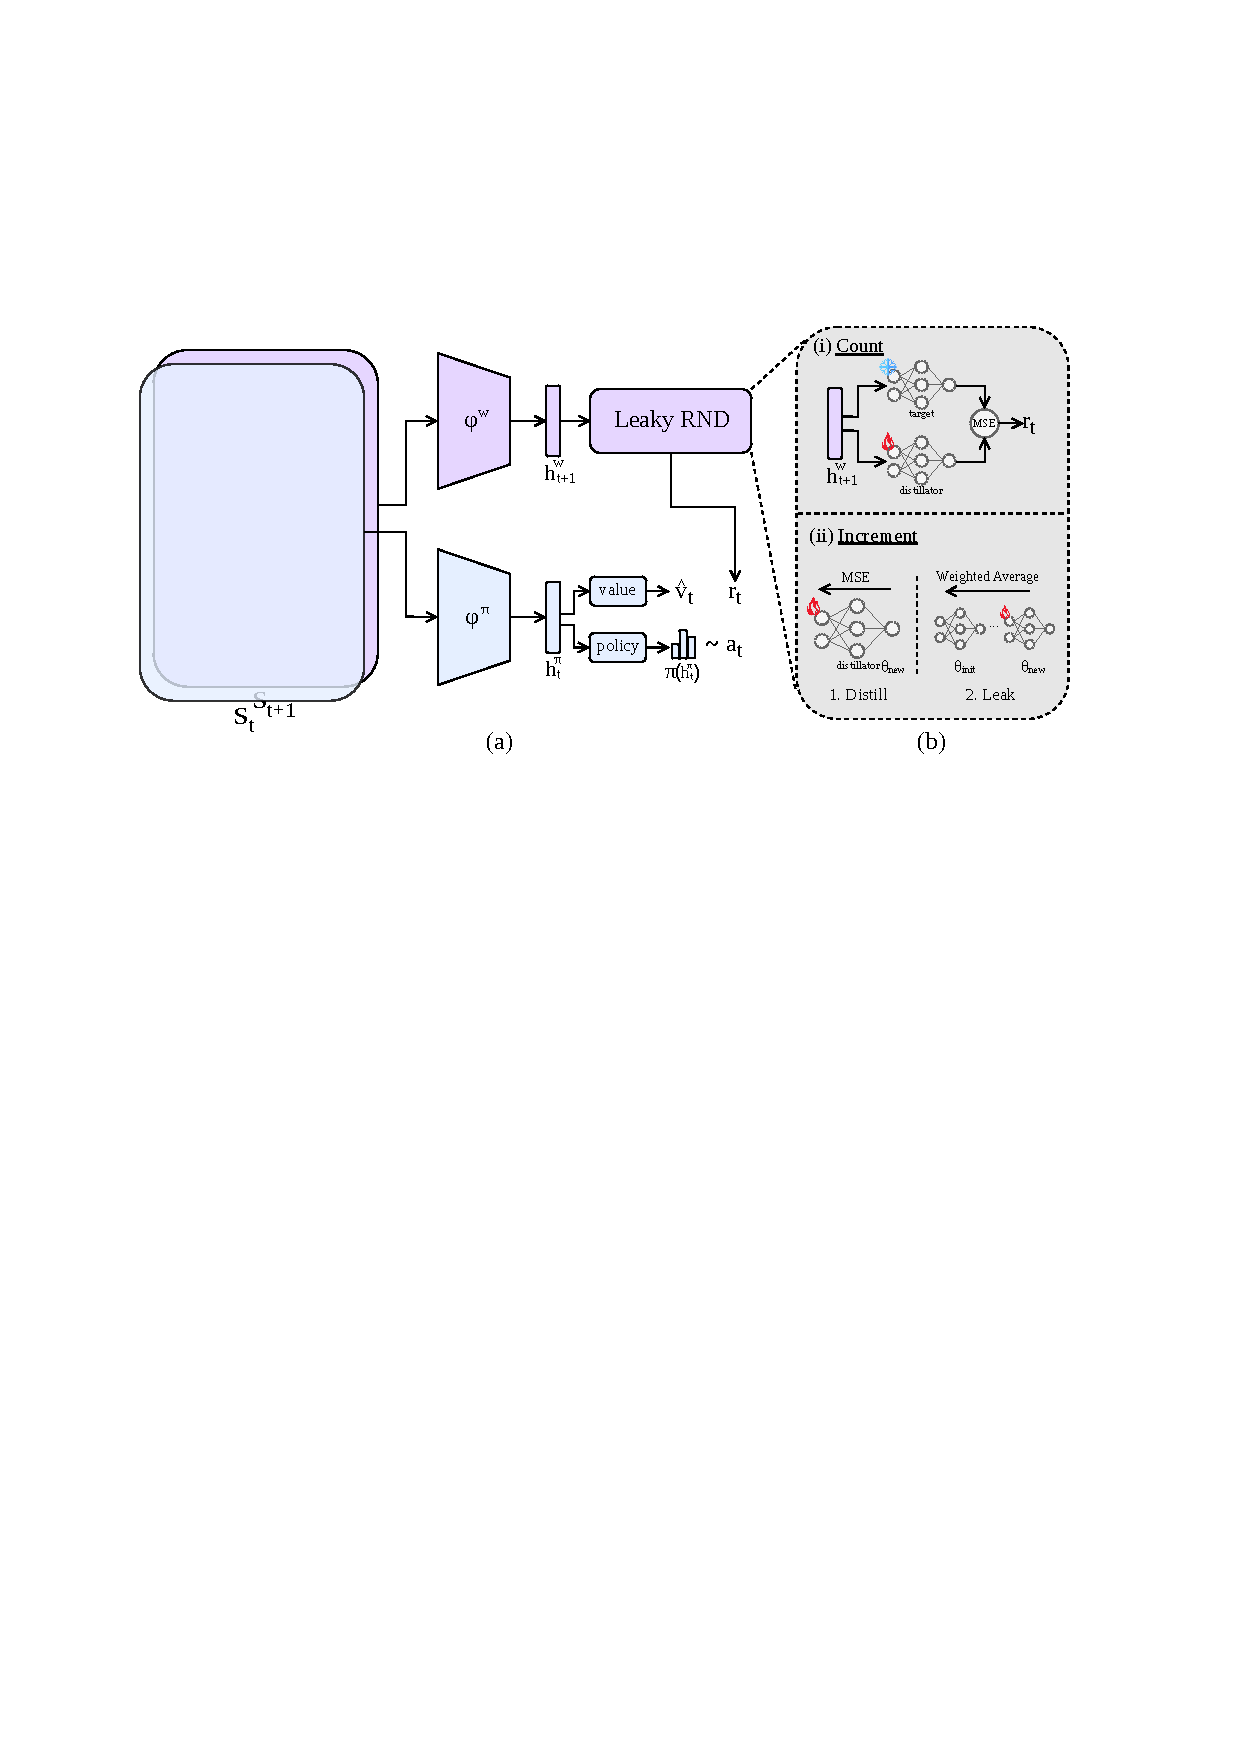
\includegraphics[width=0.9\linewidth]{LeakyRND_SystemArchitecture.drawio.pdf}
  \caption{System overview. The agent (blue) observes the current state $s_t$ and chooses an action $a_t$. The harness (purple) steps the environment, counts (b)(i) how many times $s_{t+1}$ is visited, produces a reward $r_t$ for the agent, and increments $s_{t+1}$'s visit count.}
  \label{fig:system}
\end{figure}


\subsection{Exploration in Reward-Sparse Environments}
Reinforcement Learning (RL) methods allow agents to learn from interacting with the environment, using environment feedback to improve their behavior. However, obtaining a reward in the first place can be a non-trivial task for a randomly initialized agent. Human demonstration data \citep{hester_deep_2017, salimans_learning_2018} can be used to warm-start the agent. Yet, we ultimately envision agents capable of learning on their own, in any environment, without human assistance.

Current approaches mainly drive exploration through intrinsic rewards that favor novel or unexplored states. They differ primarily in how they quantify the degree to which a state has been explored, and can be grouped into two families: count-based and prediction-based methods.

\paragraph{Count-based methods.} Count-based methods \citep{bellemare_unifying_2016, burda_exploration_2018, ostrovski_count-based_2017} track how many times each state is visited, treating more visits as better explored. A core challenge is state representation --- it's undesirable to overcount distinct observations (e.g., game screenshots) that map to the same underlying state. Pseudo-count \citep{bellemare_unifying_2016} addresses this via a density model that generalizes counts across similar states, while RND \citep{burda_exploration_2018} leverages interpolation between similar states when distilling a random network.

\paragraph{Prediction-based methods.} Prediction-based methods \citep{pathak_curiosity-driven_2017, burda_large-scale_2018, achiam_surprise-based_2017} utilize tasks like predicting the state transition, assuming better task performance at a state means more familiarity with that state. Recent works aim to tackle the noisy-TV problem \citep{burda_large-scale_2018}, where agents reward hack by fixating on states with stochastic transitions --- hence prediction error never decreases. ICM \citep{pathak_curiosity-driven_2017} introduced an inverse dynamic model so that prediction is made in a state space unaffected by uncontrollable noise, while Disagreement \citep{pathak_self-supervised_2019} instead trained multiple forward dynamic models, measuring the variance between their predictions rather than the prediction error itself.

\subsection{ARC-AGI-3}
ARC-AGI-3 \citep{foundation_arc-agi-3_2026} is a benchmark that evaluates an agent's ability to explore and plan in unseen environments. Each environment is a $64\times64$ grid-world puzzle composed of multiple levels of increasing difficulty. The only feedback an agent receives is whether it has completed a level, making the reward extremely sparse. Compounding this, solving a level often requires executing a specific sequence of actions exactly, so the probability that a random agent stumbles onto a solution decays exponentially with the length of that sequence. Frontier models like GPT-5.5 and Opus 4.7 reportedly score only 0.43\% and 0.18\% \citep{noauthor_analyzing_nodate}, confirming ARC-AGI-3 as a demanding testbed for exploration under sparse reward.

% ============================================================
\section{Methodology}
% ============================================================

Our system can be viewed as an agent with a harness. As shown in Figure~\ref{fig:system}, the agent (blue) observes the state $s_t$ and chooses an action $a_t$. The harness (purple) steps the environment, and produces a reward $r_t$ for the agent.

\subsection{Harness}
The harness consists of two modules: a world encoder $\phi^w$ that maps the game screenshot (raw pixels) $s_{t+1}$ to a hidden representation $h_{t+1}^w$; and Leaky RND, which approximates the number of times $h_{t+1}^w$ is visited with a distillation loss $\mathcal{L}_{\text{Distill}}$.

\subsubsection{World Encoder}

\begin{figure}[H]
  \centering
  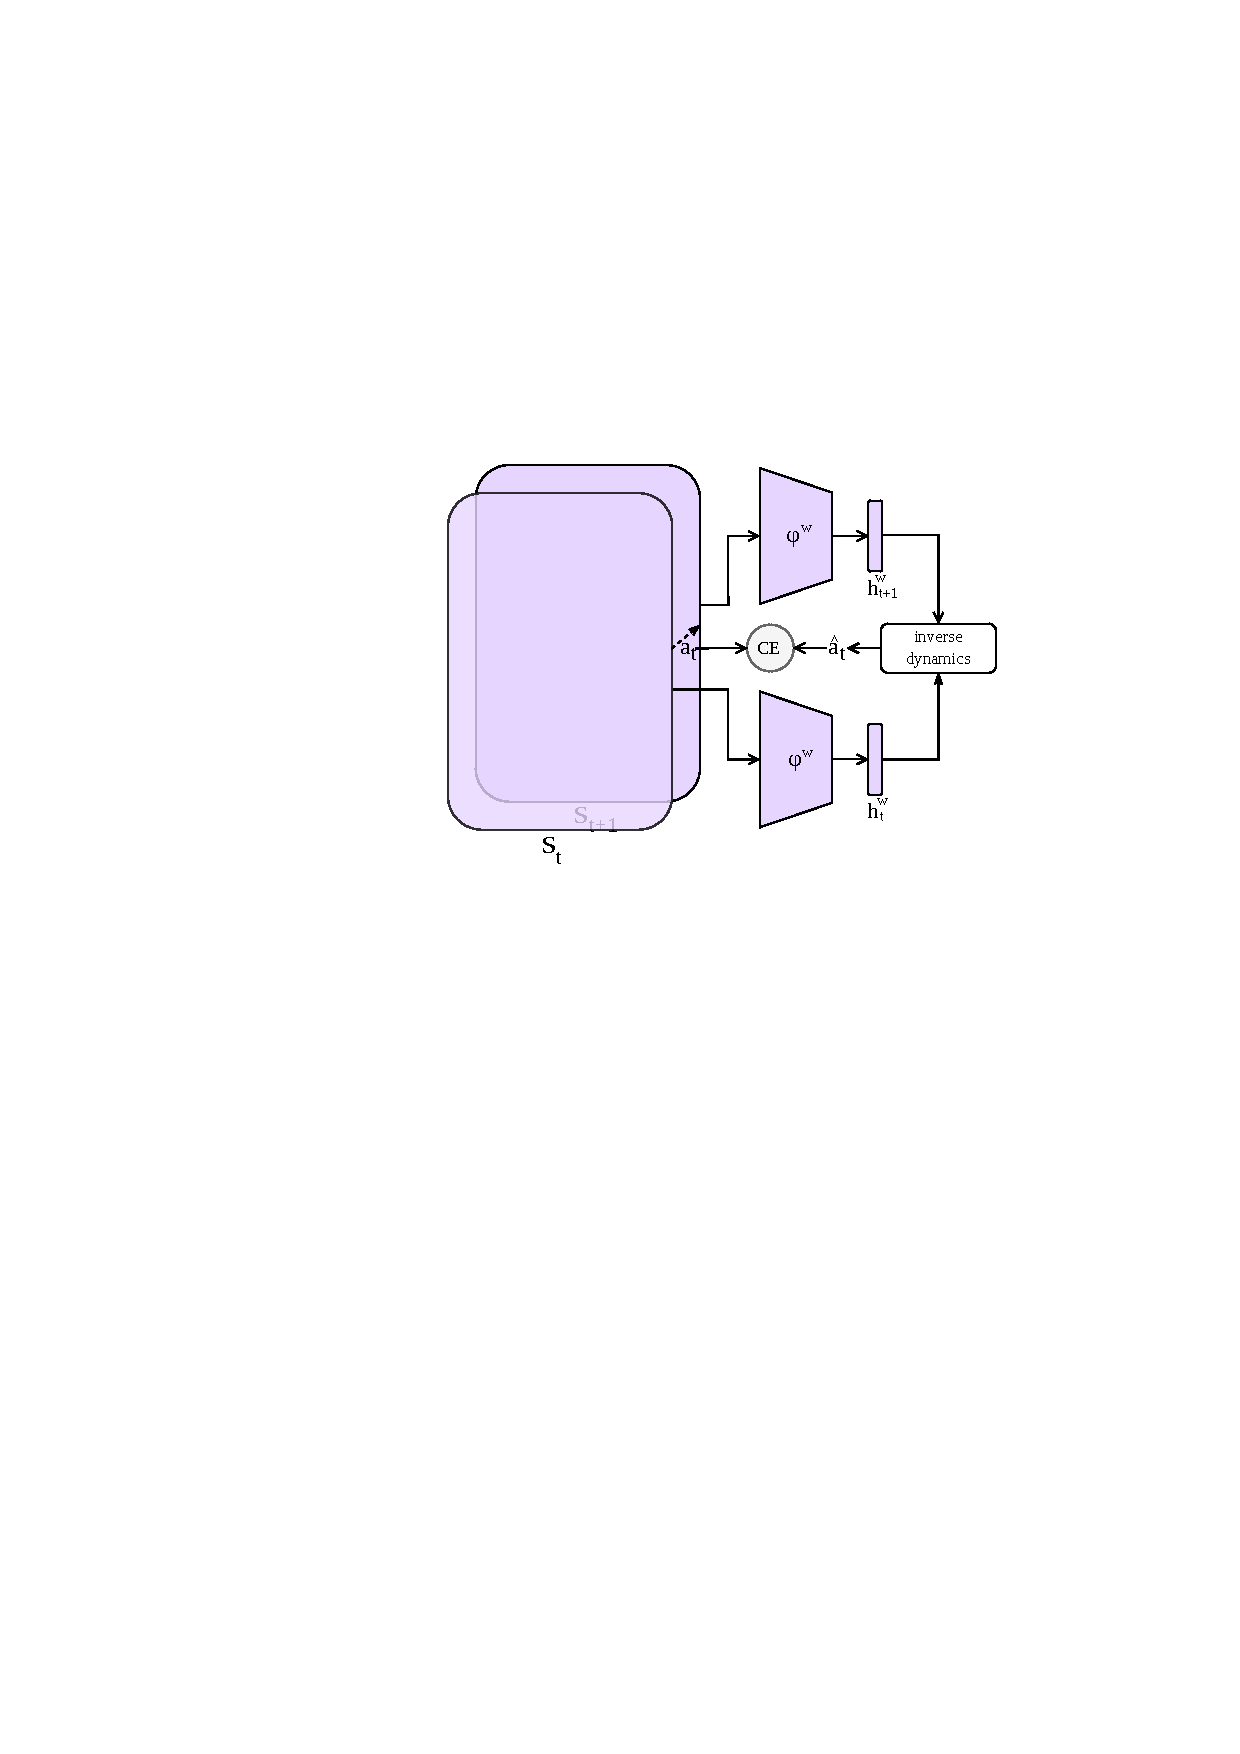
\includegraphics[height=0.22\textheight]{LeakyRND_WorldEncoder.drawio.pdf}
  \caption{World encoder trained with an inverse-dynamics objective.}
  \label{fig:encoder}
\end{figure}

\paragraph{Issue of raw pixels.} We ultimately wish to count how many times each distinct state has been visited. Counting directly in pixel space is undesirable: two frames can carry the same task-relevant information yet differ in pixels (e.g., the same agent position but a shorter energy bar), causing us to treat one state as many and overcount. We therefore want a representation that discards such task-irrelevant variation.

\paragraph{Learning representation with inverse-dynamics.} To obtain this representation, we train a world encoder $\phi^w$ with an inverse-dynamics objective (Figure~\ref{fig:encoder}). For each transition $(s_t, a_t, s_{t+1})$, we encode both states and ask an inverse-dynamics head $\text{IDM}$ to predict the action $\hat{a}=\text{IDM}(\phi^w(s_t),\phi^w(s_{t+1}))$ that produced the transition, optimized with
\begin{equation}
\mathcal{L}_{\text{IDM}} = \text{CrossEntropy}\big(\hat{a}_{t}; a_t\big)
\label{eq:idm}
\end{equation}
Such formulation forces $\phi^w$ to keep only what the agent can control and ignore the rest, so frames that differ only in task-irrelevant pixels collapse to the same representation and are no longer overcounted.

\paragraph{Online training.} $\phi^w$ is trained alongside the agent, improving as the agent explores more states. Due to this, the same state $s_t$ can be mapped to different representations $h_t^w$ as training progresses, effectively resetting the count of $s_t$. To address this, we warm-start $\phi^w$ with 20 episodes of data collected with a random policy, and treat subsequent encoder drifts (empirically small) as a natural source of leakage. Following \citet{burda_large-scale_2018}, we also tested a random encoder frozen at start, and presented the results in Section~\ref{sec:counting}.

\subsubsection{Leaky RND}
Leaky RND is used to keep track of how many times each $h_t^w$ is visited, and generate reward for the agent. Leaky RND is comprised of two modules: a randomly initialized distillation target $f_\psi$ and a distillator $\hat{f}_\theta$.

\paragraph{Counting number of visits.} $f_\psi$ assigns each state $h_t^w$ a random vector $f_\psi(h_t^w)$. Each time the agent visits a state $h_t^w$, the distillator $\hat{f}_\theta$ is allowed to distill $f_\psi$ on that state (Figure~\ref{fig:system}(b)(ii)) via
\begin{equation}
\mathcal{L}_{\text{Distill}} = \text{MSE}\big(\hat{f}_{\theta}(h_{t}^w); f_{\psi}(h_{t}^w)\big)
\label{eq:distill}
\end{equation}
The more the agent visits a state $h_t^w$, the better $\hat{f}_{\theta}$ is at distilling $f_{\psi}$ at that state. Hence, distillation error can be used as a curiosity signal (Figure~\ref{fig:system}(b)(i)): an action $a_t$ leading to a less-visited state $h_{t+1}^w$ receives a higher reward $r_t = \mathcal{L}_{\text{Distill}}(h_{t+1}^w)$ due to the higher distillation error. In practice, because $|\mathcal{L}_{\text{Distill}}|$ can vary greatly as more distillation is done, we normalize it using running statistics.

\paragraph{Curiosity saturation.} A key limitation of vanilla RND is that distillation error tends to saturate toward zero as states are visited repeatedly, eliminating the curiosity signal entirely. This is especially severe in small or structured state spaces like ARC-AGI-3, where the agent exhausts novel states quickly. Standard mitigations such as reducing $\hat{f}_\theta$'s capacity or lowering its learning rate $\eta$ can delay saturation, but do not fundamentally resolve it --- the signal eventually collapses regardless.

\paragraph{Leak mechanism.} To continuously regenerate curiosity, we introduce a leak mechanism that periodically pulls the distillator's parameters back toward their random initialization. After each distillation step, we update (Figure~\ref{fig:system}(b)(ii)):
\begin{equation}
\theta_{\text{new}}=(1-\mu)\cdot\theta_{\text{new}}+\mu \cdot \theta_{\text{init}}
\label{eq:leak}
\end{equation}
where $\mu = 0.05$ controls the degree of leak. This formulation acts as a soft reset --- gradually increasing distillation error for states that have not been recently visited, thereby restoring their curiosity signal. The intuition is that revisiting previously explored states under a new policy may yield genuinely novel behavior.

\subsection{Agent}
The agent consists of a Convolutional Neural Network (CNN) \citep{krizhevsky_imagenet_2012-1} backbone $\phi^\pi$ and a policy and a value head, trained via Proximal Policy Optimization (PPO) \citep{schulman_proximal_2017}. Detailed training setup is presented in Appendix~\ref{app:training}.

\paragraph{Intrinsic reward.} The agent is trained purely on the intrinsic reward $r_t$ supplied by the harness. Training is stopped when the agent receives its first extrinsic reward (i.e., completes a level). We experimented with transferring the learned $\phi^w$ to the next level. However, we observed it leads to minimal gains, because even though feature detectors can be reused, $\phi^w$ is unable to learn the (more conceptual) game mechanisms (e.g., being in the way of an orange blob will be eaten) shared between levels.

\paragraph{Agent-specific encoder.} We trained separate encoders $\phi^\pi$ and $\phi^w$ for the agent and the harness, since they need to perform fundamentally different tasks. We observed that a shared encoder leads to degraded performance due to gradient interference between $\mathcal{L}_{\text{IDM}}$ and $\mathcal{L}_{\text{PPO}}$.

% ============================================================
\section{Results}
% ============================================================

\subsection{Leaky RND Regenerates Curiosity}

\begin{figure}[t]
  \centering
  \begin{subfigure}[t]{0.49\linewidth}
    \centering
    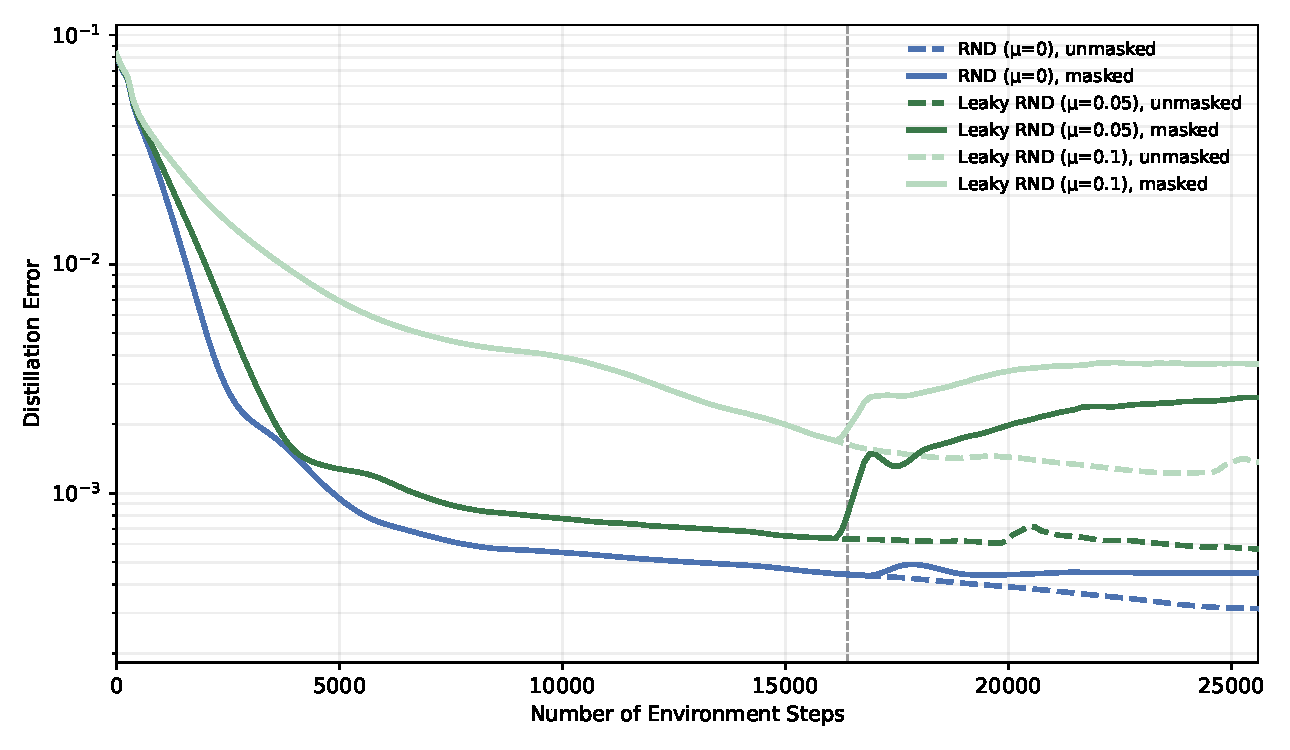
\includegraphics[height=4.2cm]{organic_forget_ls20_L2_combined.pdf}
    \caption{Distillation error of a single monitored state under RND and Leaky RND, before and after it is masked from further visits.}
    \label{fig:regen}
  \end{subfigure}
  \hfill
  \begin{subfigure}[t]{0.49\linewidth}
    \centering
    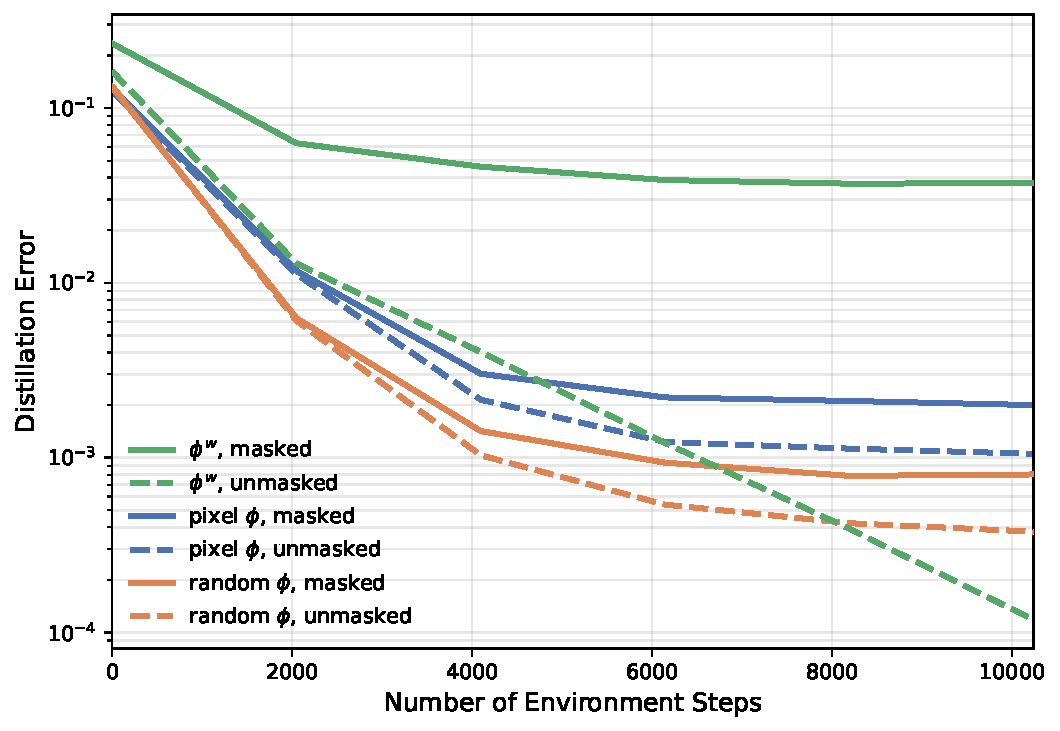
\includegraphics[height=4.2cm]{distill_error_probe_ls20_L2_seed0.pdf}
    \caption{Distillation error under pixel $\phi$, random $\phi$, and $\phi^w$ for a masked, never-visited state (solid) and a normally-visited state (dashed).}
    \label{fig:repr}
  \end{subfigure}
  \caption{Probing the curiosity signal of Leaky RND on \texttt{ls20} level 2.}
  \label{fig:probe}
\end{figure}

To study the behavior of Leaky RND, we monitored the distillation error of a single frequently-visited state near the agent's spawn in \texttt{ls20} level 2, using a frozen pre-trained world encoder $\phi^w$ to eliminate confounds. Figure~\ref{fig:regen} shows that as the agent repeatedly visits this state, its distillation error dropped and plateaued, and a higher $\mu$ saturates slower.

At ${\sim}16{,}000$ steps (128 updates), we masked actions that can reach the monitored state, so that it is no longer visited (solid lines). For vanilla RND (blue), the curiosity for the state stays low, regardless of whether it's visited (dashed) or not (solid). In contrast, with Leaky RND (green), curiosity for the state quickly regenerates as the state becomes unvisited (green, solid).

Nonetheless, the regeneration is smaller (i.e., less differentiation between visited and recently-unvisited states) for a larger $\mu$ (light green), due to a higher curiosity floor (light green, dashed). Hence, we used $\mu=0.05$ for all subsequent experiments.

\subsection{Counting in Representation Space}
\label{sec:counting}

The reliability of count-based exploration hinges on the space in which states are counted: if distinct states map to nearby representations, novelty leaks between them and the count becomes meaningless. To test this, we ran Leaky RND on three encoders --- pixel $\phi$ (raw pixels), random $\phi$ (a randomly initialized CNN, following \citep{burda_large-scale_2018}), and $\phi^w$ (warm-started) --- tracking the distillation error of a masked, never-visited state (solid) against a normally-visited one (dashed) (Figure~\ref{fig:repr}).

Under pixel $\phi$ (blue) and random $\phi$ (orange), the masked state's error falls almost as fast as the visited state's: both encoders map visually similar but distinct states to nearby representations, allowing the distillator to interpolate from visited states to unvisited ones. Counting in $\phi^w$ removes this leakage. Because inverse-dynamics training forces distinct states apart, the masked state retains a high error throughout (green, solid) while the visited state's decays (green, dashed) --- a persistent gap that distinguishes unvisited from explored states, and the prerequisite for a usable count.

\begin{figure}[H]
  \centering
  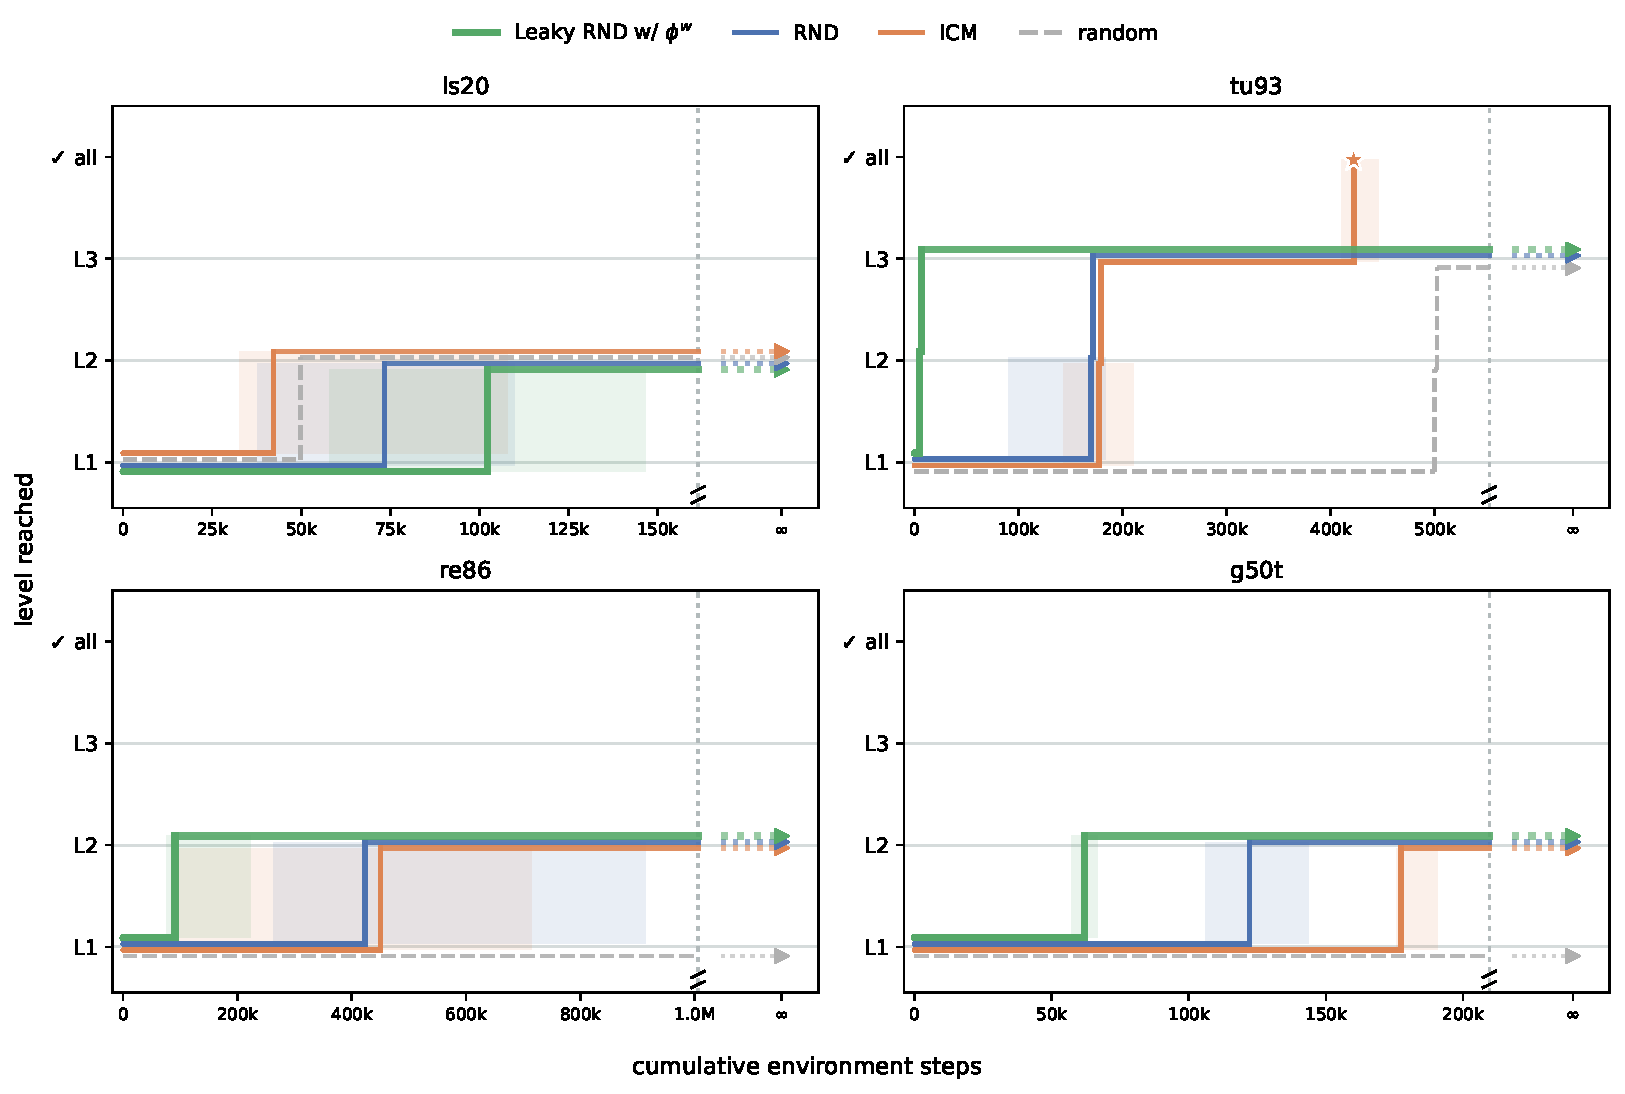
\includegraphics[width=0.9\linewidth]{main_results_grid.pdf}
  \caption{Cumulative environment steps each method requires to reach a given level, across four ARC-AGI-3 environments.}
  \label{fig:steps}
\end{figure}

\subsection{More Efficient Exploration with Leaky RND}

We evaluated our method on four environments from ARC-AGI-3's public dataset \citep{foundation_arc-agi-3_2026} (Appendix~\ref{app:envs}), reporting the average number of environment steps to complete each level against RND (blue) \citep{burda_exploration_2018} and ICM (orange) \citep{pathak_curiosity-driven_2017}. To isolate the effect of the intrinsic reward, we fixed the agent's architecture and vary only the harness that generates the reward.

Across the environments, we see ${\sim}35\%$ average reduction of steps compared to the best performing baseline. However, Leaky RND is unable to solve any of the levels previous methods couldn't solve. The main challenge is that solving these levels requires exploiting the information collected through exploration, which is missing from existing methods (further discussed in Section~\ref{sec:needed}).

\subsection{Ablation Study}
\label{sec:ablation}

\begin{table}[H]
  \centering
  \caption{\textbf{Component ablation} on four ARC-AGI-3 games (level one). Cells are the median environment steps to first reward over four seeds (lower is better).}
  \label{tab:ablation}
  \begin{tabular}{lcccc}
    \toprule
    Variant & \texttt{ls20} & \texttt{tu93} & \texttt{re86} & \texttt{g50t} \\
    \midrule
    \textbf{Full} (Leaky RND on $\phi^w$) & \textbf{32k} & 132k & \textbf{70k} & 56k \\
    \quad $-$ leak (vanilla RND) & 92k & 292k & 269k & \textbf{28k} \\
    \quad $-\,\phi^w$ (random $\phi$) & 43k & \textbf{70k} & 474k & 68k \\
    \quad $-\,\phi^w$ (pixel $\phi$) & 61k & 149k & 356k & 98k \\
    \midrule
    $-$ harness (random policy) & 50k & 500k & 1M+ & 1M+ \\
    \bottomrule
  \end{tabular}
\end{table}

We ablated the two main components of our method: the leak mechanism and the state representation $\phi^w$ (Table~\ref{tab:ablation}). Without the leak ($\mu=0$), the agent uses roughly $2$--$4\times$ more steps to solve a level on \texttt{ls20}, \texttt{tu93}, and \texttt{re86}, confirming that continuously regenerating curiosity accelerates exploration. The exception is \texttt{g50t}, where eliminating the leak improves performance, presumably because its large number of distinct states makes forgetting which states have been visited harmful for exploration.

Switching $\phi^w$ to a randomly initialized encoder or a raw-pixel encoder consistently degrades performance, with \texttt{tu93} as the lone exception. Finally, ablating the harness entirely removes the intrinsic reward, leaving the agent no learning signal and reducing it to random exploration. This baseline never solves \texttt{re86} or \texttt{g50t} within 1M steps and is slower than Leaky RND on the two levels it does clear, confirming that the intrinsic reward, rather than chance, drives exploration.

% ============================================================
\section{Discussion}
% ============================================================

\subsection{What is needed for ARC-AGI-3}
\label{sec:needed}
Reflecting on our results, we believe that achieving progress on ARC-AGI-3 necessitates two things: general knowledge and intentionality.

\paragraph{General knowledge.} Humans build their understanding of game mechanisms on top of concepts (e.g., clicking on a grid will attract nearby blobs toward it). Concepts carry associations and do the heavy weight-lifting during generalization. An agent solely trained on ARC-AGI-3 will not be exposed to this wide variety of concepts they can leverage to describe and model the world. They have to build their abstractions from scratch, and if they are in the form of opaque world models, then they further miss out the opportunity to utilize the priors human built.

\paragraph{Intentionality.} Existing methods explore blindly. Humans, by contrast, explore with intent: we use what we observe to infer how a game works, then direct our actions accordingly (e.g., move to the bottom-left to test what the yellow blob does). This matters because completing a level often demands a specific action sequence (e.g., reach the cross, refill energy, reach the exit). Curiosity-based exploration has no mechanism for composing such structure. More fundamentally, it never exploits the information it gathers, lacking the reasoning capability to do so.

Hence, we believe general agents will emerge from LLMs, inheriting from language the priors needed for exploration, planning, and understanding.

\subsection{Count-based exploration as implicit MCTS}
Monte Carlo Tree Search (MCTS) works by using rollouts to iteratively refine value estimates of states. During rollouts, exploration and exploitation is balanced with UCT \citep{hutchison_bandit_2006}. We realized that exploration with count-based bonuses can be interpreted as an amortized version of MCTS.

During action selection, the agent is rewarded for both exploitation (extrinsic reward) and exploration (count-based bonus), where the balance is implicitly represented in the policy. Alternatively, one can explicitly compute the UCT score and use that to guide action selection, armed with visit-counters like RND and other methods. One episode can be treated as a single rollout, where the terminal reward (leaf node value) is propagated upward through visited states via value function updates. Thus, count-bonus exploration amounts to a degenerate MCTS that searches a single tree with no explicit lookahead --- explaining both its sample efficiency and its inability to plan toward distant goals.

% ============================================================
\section{Conclusion}
% ============================================================
In this work, we introduced Leaky RND, a count-based exploration method that prevents curiosity saturation by periodically pulling the distillator's parameters toward their random initialization, leaking information so that curiosity is restored for states not visited recently. We demonstrated that a representation space learned through inverse-dynamics modeling is better suited to count-based exploration than a random feature space, particularly when distinct states are visually similar. Our method completes a level in roughly 35\% fewer steps than the best baseline. However, it cannot solve any level that existing methods cannot. We argue that this reflects a fundamental limitation of curiosity-based exploration: it lacks the intentionality needed to direct exploration and act on the information it gathers. We believe a general agent capable of progressing on ARC-AGI-3 will need to emerge from LLMs, drawing on the vast priors and abstractions that humans have encoded in language.

% ============================================================
\bibliographystyle{plainnat}
\bibliography{cse190_lib}
% ============================================================

\appendix

\section{Training Setup}
\label{app:training}

\subsection{Observation and Action Space}
\label{app:obs}
Each observation is a $64\times64$ grid of ARC palette indices over
$n_{\text{colors}}=16$ colors. We one-hot encode each grid into a
$16\times64\times64$ tensor and apply no resizing, frame stacking, or cropping.
The action space is the discrete ARC-AGI-3 action set; the per-environment
action sets are listed in Appendix~\ref{app:envs}. Each run trains on a single level; episodes start from that
level's initial state and end on completion or at a $200$-step horizon,
whichever comes first. The environment emits an extrinsic reward of $+1$ only on
completion. This signal is never given to the agent; it is used solely to mark
when a level is solved for the steps-to-solve metric (Appendix~\ref{app:protocol}).

\subsection{Network Architectures}
\label{app:arch}
The agent encoder $\phi^\pi$ and the world encoder $\phi^w$ are two independent
instances of the same convolutional architecture (Table~\ref{tab:cnn}); they
share neither weights nor gradients. The inverse-dynamics (IDM) head, the RND
target $f_\psi$, and the distillator $\hat{f}_\theta$ all operate on the
$256$-dimensional world representation $h^w$ produced by $\phi^w$
(Table~\ref{tab:heads}). All layers use orthogonal initialization --- gain
$\sqrt{2}$, except the policy head ($0.01$) and the value head ($1.0$) --- with
ReLU activations and no normalization or pooling.

\begin{table}[h]
\centering
\caption{Shared CNN encoder. Input $16\times64\times64$ one-hot frame; output a
$256$-d feature vector. Used independently for $\phi^\pi$ and $\phi^w$.}
\label{tab:cnn}
\begin{tabular}{lccccc}
\toprule
Layer & Type & Out ch. & Kernel & Stride & Pad \\
\midrule
1 & Conv2d + ReLU & 32 & 3 & 1 & 1 \\
2 & Conv2d + ReLU & 64 & 3 & 2 & 1 \\
3 & Conv2d + ReLU & 64 & 3 & 2 & 1 \\
4 & Conv2d + ReLU & 64 & 3 & 2 & 1 \\
  & Flatten       & \multicolumn{4}{c}{$64\times8\times8 = 4096$} \\
5 & Linear + ReLU & \multicolumn{4}{c}{$4096 \to 256$ (trunk)} \\
\bottomrule
\end{tabular}
\end{table}

\begin{table}[h]
\centering
\caption{Heads. Policy/value heads sit on $\phi^\pi$; the IDM head and Leaky RND
networks sit on $\phi^w$. $d=256$ is the trunk/world-representation dim.}
\label{tab:heads}
\begin{tabularx}{\linewidth}{l >{\raggedright\arraybackslash}X l}
\toprule
Module & Architecture & Notes \\
\midrule
Policy head        & $\text{Linear}(d\to|\mathcal{A}|)$ & gain $0.01$ \\
Value head         & $\text{Linear}(d\to 1)$            & gain $1.0$ \\
IDM head           & $\text{Linear}(2d\to256)$, ReLU, $\text{Linear}(256\to|\mathcal{A}|)$ & predicts $\hat a_t$ \\
RND target $f_\psi$      & $\text{Linear}(d\to256)$, ReLU, $\text{Linear}(256\to256)$ & frozen at init \\
RND distillator $\hat f_\theta$ & $\text{Linear}(d\to256)$, ReLU, $\text{Linear}(256\to256)$, ReLU, $\text{Linear}(256\to256)$ & trainable (deeper than target) \\
\bottomrule
\end{tabularx}
\end{table}

\subsection{World Encoder $\phi^w$}
\label{app:worldenc}
We train $\phi^w$ solely with the inverse-dynamics objective of
Equation~\eqref{eq:idm}, propagating no PPO gradient into it, using a dedicated
Adam optimizer (Table~\ref{tab:wenc}). Before the main loop, we warm-start
$\phi^w$ on transitions from $20$ random-policy episodes, so that novelty is
measured in a stable representation from the outset rather than in that of a
freshly initialized encoder. These warm-up steps count toward both the step
budget and the steps-to-solve metric. During training, $\phi^w$ continues to
update online alongside the agent; the resulting representational drift is small
and acts as a natural source of leakage.

\begin{table}[h]
\centering
\caption{World-encoder training hyperparameters.}
\label{tab:wenc}
\begin{tabular}{ll}
\toprule
Hyperparameter & Value \\
\midrule
Optimizer & Adam, lr $1\times10^{-3}$ \\
World representation dim $|h^w|$ & $256$ \\
IDM hidden width & $256$ \\
Warm-start episodes (random policy) & $20$ \\
Warm-start epochs / batch size & $4$ / $256$ \\
Online update & one pass per PPO update, gradient clip $0.5$ \\
\bottomrule
\end{tabular}
\end{table}

\subsection{Leaky RND}
\label{app:leakyrnd}
Leaky RND scores the raw novelty of a state as
$\tfrac{1}{2}\,\text{mean}_j\big(\hat f_\theta(h^w)_j - f_\psi(h^w)_j\big)^2$, the
mean squared distillation error between the distillator $\hat f_\theta$ and the
frozen target $f_\psi$, and updates $\hat f_\theta$ toward $f_\psi$ by minimizing
$\mathcal{L}_{\text{Distill}}$ (Equation~\ref{eq:distill}). After each
distillation minibatch, we apply the leak update of Equation~\eqref{eq:leak} with
$\mu = 0.05$, pulling $\hat f_\theta$ back toward its random initialization.
Transitions whose successor is a reset state are excluded from both the novelty
bonus and the distillation update. Table~\ref{tab:leaky} lists all
hyperparameters.

\paragraph{Reward normalization.} We map raw novelty to the intrinsic reward
using running statistics, with three stabilizing measures. (i) The agent
receives no intrinsic reward during the first $2$ PPO updates, letting the
distillator reach a stable error scale before its output drives the policy.
(ii) We divide raw novelty by an exponential moving average (EMA, decay $0.99$)
of the standard deviation of the discounted intrinsic returns, applying no
mean-centering so the bonus stays non-negative; we use an EMA rather than a
cumulative estimate because the leak renders the novelty signal non-stationary.
(iii) We clip per-step raw novelty at $5\times$ its running mean before
normalization, preventing transient spikes from corrupting the return
statistics.

\begin{table}[h]
\centering
\caption{Leaky RND hyperparameters.}
\label{tab:leaky}
\begin{tabular}{ll}
\toprule
Hyperparameter & Value \\
\midrule
Target / distillator output dim & $256$ \\
Distillator optimizer & Adam, lr $\eta = 1\times10^{-4}$ \\
Distillation passes per update & $1$ (over rollout, $4$ minibatches) \\
Leak rate $\mu$ & $0.05$ \\
Leak cadence & after each distillation minibatch step \\
Normalization warm-up (updates) & $2$ \\
Intrinsic-return EMA decay & $0.99$ \\
Raw-novelty clip & $5\times$ running mean \\
\bottomrule
\end{tabular}
\end{table}

\subsection{Agent and PPO}
\label{app:ppo}
The agent is the convolutional actor-critic of Table~\ref{tab:cnn}, with separate
policy and value heads, trained by PPO on the normalized intrinsic reward alone.
Because each run stops at the first extrinsic reward, we use a single value head
for the intrinsic return and estimate advantages with non-episodic generalized
advantage estimation (GAE), bootstrapping across episode resets as in
RND~\citep{burda_exploration_2018}. Table~\ref{tab:ppo} lists all hyperparameters.

\begin{table}[h]
\centering
\caption{Agent / PPO hyperparameters.}
\label{tab:ppo}
\begin{tabular}{ll}
\toprule
Hyperparameter & Value \\
\midrule
Parallel environments $N$ & $16$ \\
Rollout length $T$ & $128$ ($2048$ transitions / update) \\
Optimizer & Adam, lr $3\times10^{-4}$ \\
Discount $\gamma$ (intrinsic) & $0.99$ \\
GAE $\lambda$ & $0.95$ \\
PPO clip $\epsilon$ & $0.2$ \\
Value-clip $\epsilon$ & $0.2$ \\
Epochs / minibatches per update & $4$ / $4$ \\
Value loss coefficient & $0.5$ \\
Entropy coefficient & $0.01$ \\
Gradient clip (max norm) & $0.5$ \\
Advantage normalization & per-minibatch \\
\bottomrule
\end{tabular}
\end{table}

\subsection{Training and Evaluation Protocol}
\label{app:protocol}
Training on each level terminates at the first extrinsic reward. The reported
metric is the cumulative number of environment steps up to that point, summed
across the $16$ parallel actors and inclusive of the warm-up steps. Runs that do
not solve a level within its step budget are right-censored at the cap. Each
trainable module uses its own Adam optimizer --- the agent, the world encoder
$\phi^w$ together with its IDM head, and the distillator $\hat f_\theta$ ---
while the target network $f_\psi$ remains frozen at initialization and is never
updated. Per-level step budgets and the corresponding random-policy reference are
given in Table~\ref{tab:budget}, and the evaluation environments are described in
Appendix~\ref{app:envs}.

\paragraph{Seeds and aggregation.} Seed counts vary by experiment. The main
steps-to-solve results (Figure~\ref{fig:steps}) use up to $4$ seeds
($\{0,1,2,3\}$) per (method $\times$ environment $\times$ level) cell on level~1,
with fewer on the harder upper levels; for each cell we report the median
steps-to-first-reward over the seeds that solved, with a $25$--$75$th percentile
band. The representation-space comparison (Section~\ref{sec:counting},
Figure~\ref{fig:repr}) uses $5$ seeds ($\{0,1,2,3,4\}$). The single-state
curiosity-regeneration and counting probes (Figures~\ref{fig:regen}
and~\ref{fig:repr}) use a single seed ($0$) and a single monitored state, since
they isolate one state's distillation error rather than aggregate performance.
The ablation study (Section~\ref{sec:ablation}) uses $3$ seeds ($\{0,1,2\}$).

\begin{table}[h]
\centering
\caption{Per-environment level-1 step budget (censoring cap) and the approximate
expected steps-to-first-reward of a uniform-random policy on level~1.}
\label{tab:budget}
\begin{tabular}{lccc}
\toprule
Environment & $|\mathcal{A}|$ & Level-1 step budget & Random-policy E[steps] (L1) \\
\midrule
\texttt{ls20} & 4 & $200{,}000$    & ${\sim}49{,}800$ \\
\texttt{tu93} & 4 & $600{,}000$    & ${\sim}500{,}000$ \\
\texttt{re86} & 5 & $1{,}000{,}000$ & $\infty$ (never clears) \\
\texttt{g50t} & 5 & $300{,}000$    & $\infty$ (never clears) \\
\bottomrule
\end{tabular}
\end{table}

The budgets above are for level~1; the main grid (Figure~\ref{fig:steps}) also
covers levels~2--3 under comparable per-cell caps (e.g., \texttt{ls20} level~2 at
$300{,}000$ steps). A
uniform-random policy clears \texttt{tu93} level~2 in ${\sim}2{,}200$ steps but
clears no other level shown.

Algorithm~\ref{alg:leakyrnd} summarizes the complete per-level training loop.

\begin{algorithm}[H]
\caption{Leaky RND training loop (one level)}
\label{alg:leakyrnd}
\begin{algorithmic}[1]
\State Warm-start $\phi^w$ on $20$ random-policy episodes (inverse dynamics, Eq.~\ref{eq:idm})
\For{each PPO update}
  \State Collect a rollout of $T{=}128$ steps in $N{=}16$ envs with policy $\pi$
  \State Encode successors $h^w_{t+1} = \phi^w(s_{t+1})$
  \State Raw novelty $\leftarrow \tfrac{1}{2}\,\text{mean}_j(\hat f_\theta(h^w_{t+1})-f_\psi(h^w_{t+1}))^2$; zero reset steps
  \State $r_t \leftarrow$ normalize(raw novelty) \Comment{warm-up, EMA-std, clip; Sec.~\ref{app:leakyrnd}}
  \State Estimate non-episodic GAE; update $\pi$ and value head (PPO)
  \State Update $\phi^w$ by inverse dynamics (Eq.~\ref{eq:idm}) \Comment{online}
  \For{each distillation minibatch}
    \State Step $\hat f_\theta$ on $\mathcal{L}_{\text{Distill}}$ (Eq.~\ref{eq:distill})
    \State Leak: $\theta \leftarrow (1-\mu)\,\theta + \mu\,\theta_{\text{init}}$ \Comment{$\mu=0.05$, Eq.~\ref{eq:leak}}
  \EndFor
  \State \textbf{if} an extrinsic reward was observed \textbf{then} record step and \textbf{stop}
\EndFor
\end{algorithmic}
\end{algorithm}

\section{Evaluation Environments}
\label{app:envs}

We evaluate on four environments drawn from ARC-AGI-3's public set:
\texttt{ls20}, \texttt{tu93}, \texttt{re86}, and \texttt{g50t}. ARC-AGI-3 games
are turn-based $64\times64$ grid puzzles that are presented without
instructions: the objects, rules, and win condition of each level must be
inferred purely through interaction, and each game is organized into successive
levels that introduce new mechanics. We use the games unmodified and expose the
agent to the intrinsic reward only.

\end{document}